\section{User's manual}
% o Description of how to install, compile and run the game/robot. 
% o Screenshots from the game describing how to play the game.

\subsection{Prerequisites}
The server application is hosted in the cloud and should ``just work''. You will need a stable Internet connection on your Android device/desktop computer and an opponent to play against. 

\subsection{Installation instructions}
Our goal is to make the application available through the Google Play Store. As of April 21, you can find our game published here: \url{https://play.google.com/store/apps/details?id=com.mygdx.seabattle.android}. In Play Store, the fastest way to find the game, is to search for 'Mats Byrkjeland'. 

You can also visit the GitHub page~\cite{github} for the project. Download the APK file to your Android device. Allow untrusted APKs to run on your Android device (under Settings), and install the APK.

The APK file is included in the final delivery, bundled together with a JAR file that runs in the JVM on OS X, Windows and Linux. Run the JAR file from the command line with \verb|java -jar desktop.jar|.

\subsection{Setup instructions (from scratch)}
Follow the setup instructions for the client and the server provided in README.md on the GitHub page~\cite{github}. To build for the client, you will need to use IntelliJ / Android Studio with Gradle, and choose a Desktop or Android run configuration. 

\subsection{How to play}
\begin{center}
\renewcommand{\arraystretch}{2}
\begin{longtable}{rp{7cm}r}
1. & Run two instances of the game. You will be presented with the main menu. & \raisebox{-0.95\height}{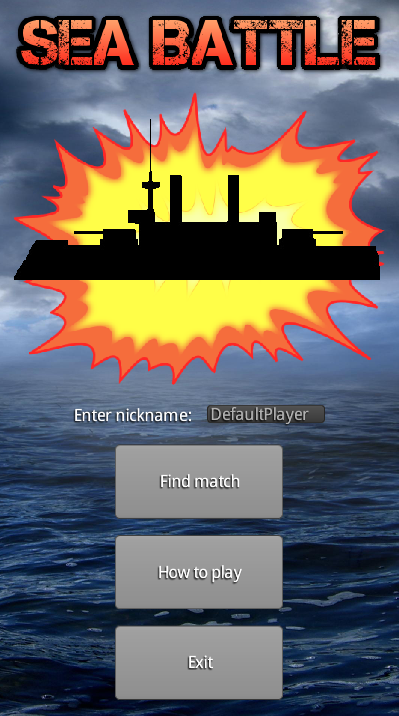
\includegraphics[scale=0.4]{figs/main-menu}} \\
2. & Click on `How to play' for instructions. & \raisebox{-0.95\height}{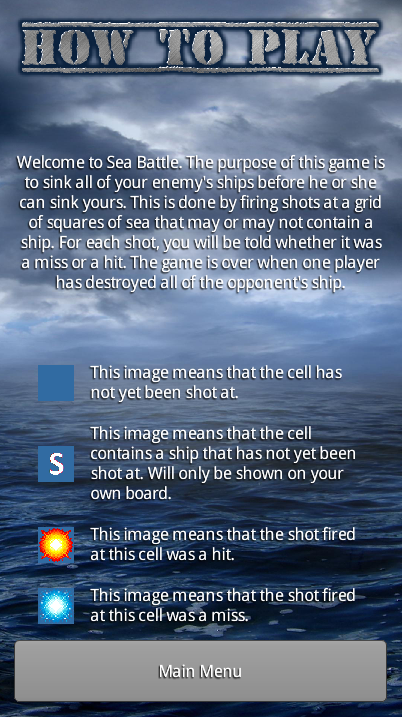
\includegraphics[scale=0.4]{figs/how-to-play}} \\
3. & Choose a player name and click on `Find match'. Wait for another player to join. & \raisebox{-0.95\height}{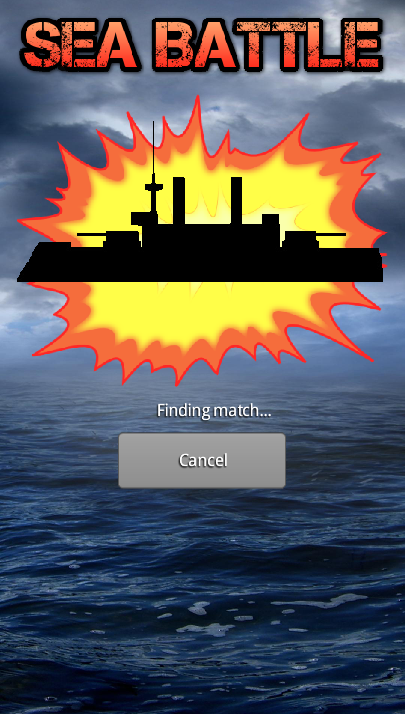
\includegraphics[scale=0.4]{figs/finding-match}} \\
4. & Wait for the opponent to fire first. & \raisebox{-0.95\height}{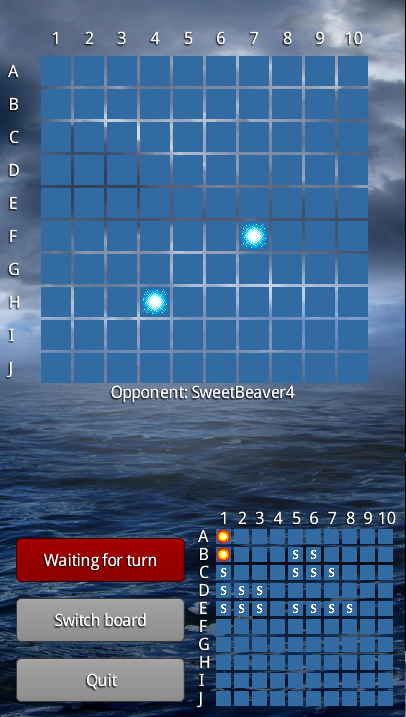
\includegraphics[scale=0.4]{figs/wait-for-turn}} \\
5. & It is now your turn to fire. Choose a board cell and press `Fire'. & \raisebox{-0.95\height}{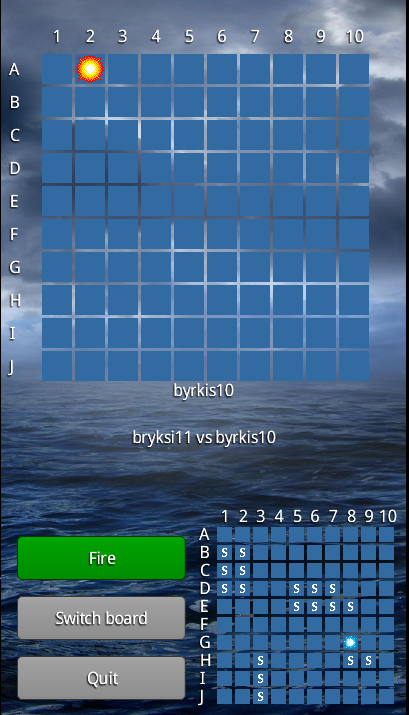
\includegraphics[scale=0.4]{figs/fire}} \\
6. & You can swap the location of the boards if you wish to see your own board in a larger frame. & \raisebox{-0.95\height}{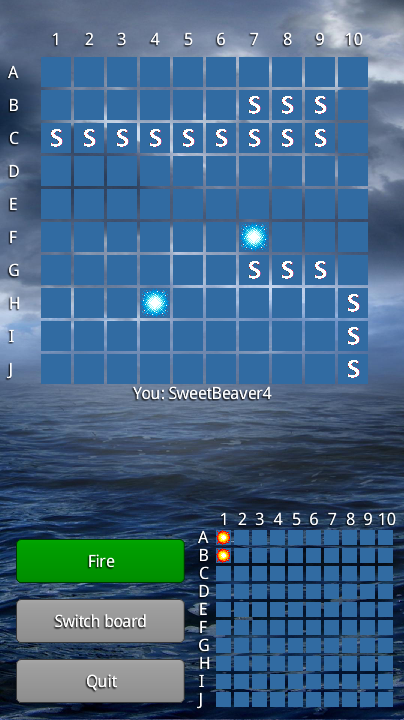
\includegraphics[scale=0.4]{figs/swapped-boards}} \\
7. & Game over. You will be notified about whether you or your opponent won. & \raisebox{-0.95\height}{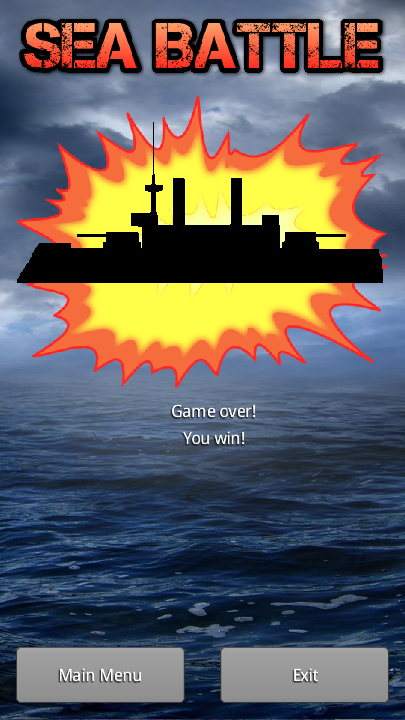
\includegraphics[scale=0.4]{figs/game-over}} \\
\end{longtable}
\end{center}
